\documentclass[../main.tex]{subfiles}

\begin{document}

\section{MOSAIC for VASO fMRI} 

\authors{Renzo (Laurentius) Huber\textsuperscript{1}, Remi Gau\textsuperscript{2}, R\"udiger Stirnberg\textsuperscript{3}, Philipp Ehses\textsuperscript{3}, \"Omer Faruk G\"ulban\textsuperscript{1,4}, Benedikt A Poser\textsuperscript{1}}

\affiliations{1. Faculty of Psychology and Neuroscience, Maastricht University, Maastricht, The Netherlands, 2.
Institute of Psychology, Universit\'{e} Catholique de Louvain, Louvain-la-Neuve, Belgium and Institute of Neuroscience, Universit\'{e} Catholique de Louvain, Louvain-la-Neuve, Belgium, 3 German Center for Neurodegenerative Diseases (DZNE), Bonn, Germany, 4. Brain Innovation, Maastricht, The Netherlands.} 

Vascular Space Occupancy (VASO) is a functional magnetic resonance imaging (fMRI) method that is used for high-resolution cortical layer-specific imaging \parencite{Huber2021a}. Currently, the most popular sequence for VASO at modern SIEMENS scanners is the one by \textcite{Stirnberg2021a} from the DZNE in Bonn, which is employed at more than 30 research labs worldwide. This sequence concomitantly acquires fMRI BOLD and blood volume signals. In the SIEMENS' reconstruction pipeline, these two complementary fMRI contrasts are mixed together within the same time series, making the outputs counter-intuitive for users. Specifically:

\begin{itemize}
    \item The 'raw' NIfTI converted time-series are not BIDS compatible (see \href{https://github.com/bids-standard/bids-specification/issues/1001}{https://github.com/bids-standard/bids-specification/issues/1001}).
    
    \item The order of odd and even BOLD and VASO image TRs is unprincipled, making the ordering dependent on the specific implementation of NIfTI converters.
\end{itemize}

Workarounds with 3D distortion correction, results in interpolation artifacts. Alternative workarounds without MOSAIC decorators result in unnecessarily large data sizes.

In the previous Brainhack \parencite{Gau2021}, we extended the existing 3D-MOSAIC functor that was previously developed by Benedikt Poser and Philipp Ehses. This functor had been previously used to sort volumes of images by dimensions of echo-times, by RF-channels, and by magnitude and phase signals. In this Brainhack, we successfully extended and validated this functor to also support the dimensionality of SETs (that is representing BOLD and VASO contrast).

We are happy to share the compiled SIEMENS ICE (Image Calculation Environment) functor that does this sorting. Current VASO users, who want to upgrade their reconstruction pipeline to get the MOSAIC sorting feature too, can reach out to Renzo Huber (RenzoHuber@gmail.com) or R\"udiger Stirnberg (Ruediger.Stirnberg@dzne.de).

\begin{figure}
	\centering
	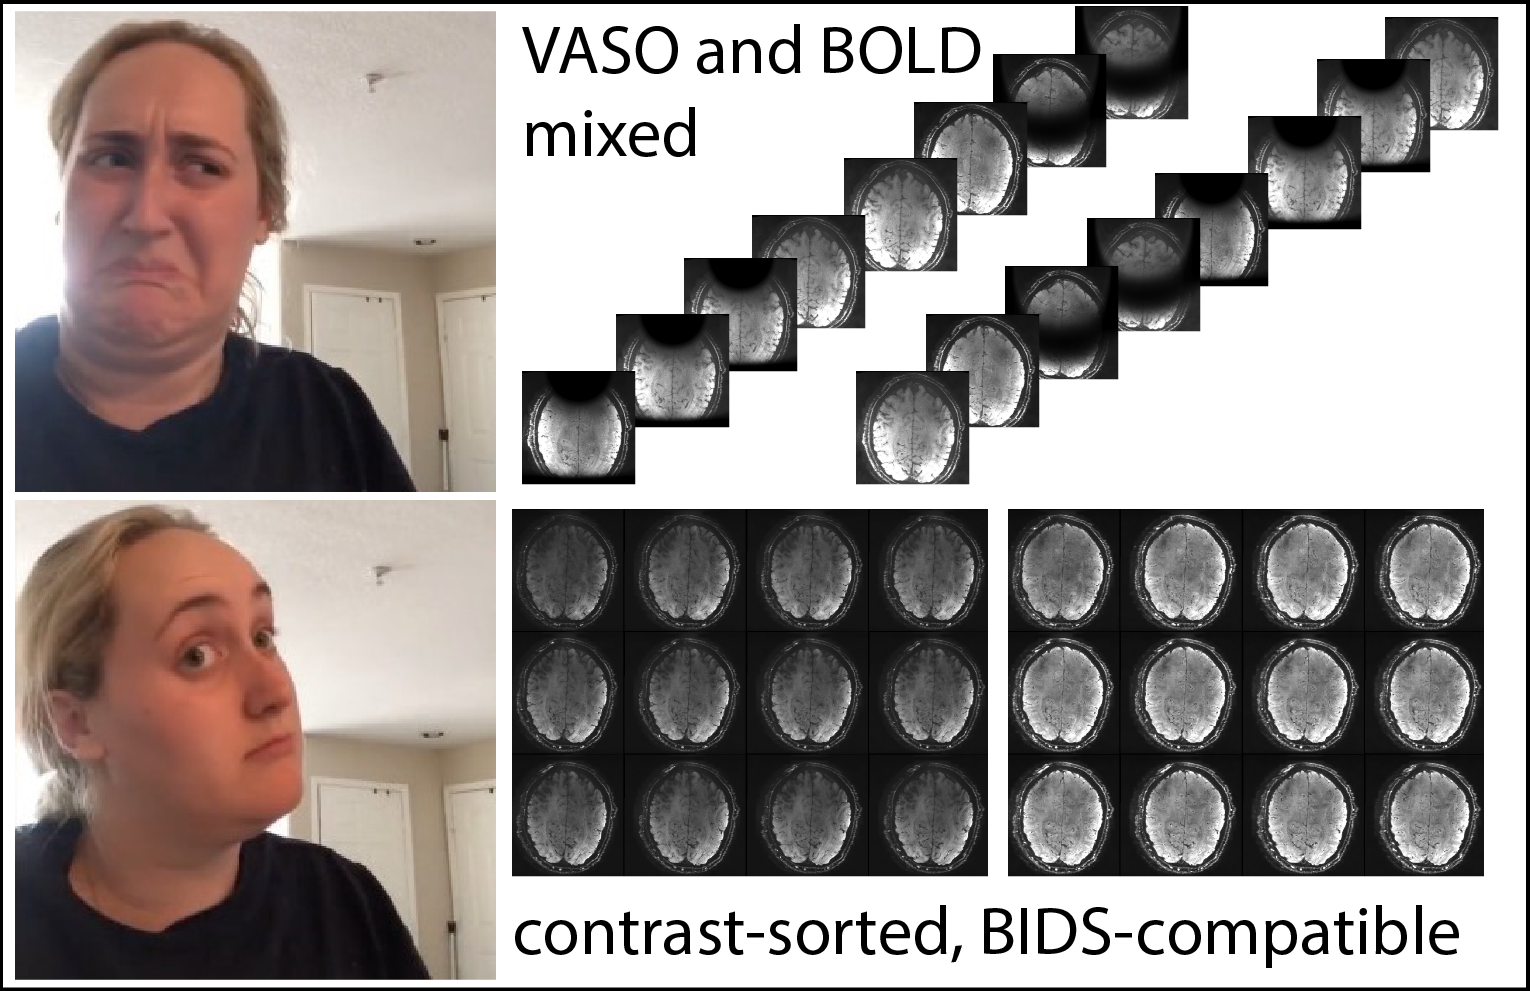
\includegraphics[width=0.5\textwidth]{VASOMOSAIC.png}
	\caption{Previously, most VASO sequences provided unsorted image series of MRI contrasts. This was not BIDS compatible and could suffer from gradient non-linearity artifacts in the scanner’s MR-reconstruction pipeline. In Brainhack 2022, we adapted the SIEMENS reconstruction and to sort volume series by fMRI contrasts. This is BIDS compatible and does not require non-linearity corrections.
}
	% Add a label to reference in text. Make it specific!
	\label{fig:VASOMOSAIC}
\end{figure}

-----------------------------------

Furthermore, Remi Gau, generated a template dataset that exemplifies how one could to store layer-fMRI VASO data. This includes all the meta data for ‘raw’ and ‘derivatives’. Link to this VASO fMRI BIDS demo: \href{https://gin.g-node.org/RemiGau/ds003216/src/bids_demo}{https://gin.g-node.org/RemiGau/ds003216/src/bids\textunderscore demo}.

-----------------------------------

Acknowledgements: We thank Chris Rodgers for instructions on how to overwrite existing reconstruction binaries on the SIEMENS scanner without rebooting. We thank David Feinberg, Alex Beckett and Samantha Ma for helping in testing the new reconstruction binaries at the Feinbergatron scanner in Berkeley via remote scanning. We thank Maastricht University Faculty of Psychology and Neuroscience for supporting this project with 2.5 hours of 'development scan time'.

\printbibliography

\end{document}
